\documentclass[12pt,letterpaper]{exam}
\usepackage[lmargin=1in,rmargin=1in,tmargin=1in,bmargin=1in]{geometry}
\usepackage{../style/exams}

% -------------------
% Course & Exam Information
% -------------------
\newcommand{\course}{MAT 108: Exam 2}
\renewcommand{\term}{Fall -- 2023}
\newcommand{\examdate}{11/09/2023}
\newcommand{\timelimit}{85 Minutes}

\setbool{hideans}{false} % Student: True; Instructor: False

% -------------------
% Content
% -------------------
\begin{document}

\examtitle
\instructions{Write your name on the appropriate line on the exam cover sheet. This exam contains \numpages\ pages (including this cover page) and \numquestions\ questions. Check that you have every page of the exam. Answer the questions in the spaces provided on the question sheets. Be sure to answer every part of each question and show all your work. If you run out of room for an answer, continue on the back of the page --- being sure to indicate the problem number.} 
\scores
\bottomline
\newpage

% ---------
% Questions
% ---------
\begin{questions}

% Question 1
\newpage
\question[10] You have purchased a race horse called Elmer G. The previous owner claims that in a race there is a $\frac{1}{14}$ chance he will come in first, a $\frac{2}{14}$ chance that he will come in second, and a $\frac{4}{14}$ chance that he will come in third. You can enter the horse in a race at a local track for \$800. The race has a \$3,000 prize for first place, a \$2,000 prize for second place, and a \$1,000 prize for third place. 
	\begin{enumerate}[(a)]
	\item Find the probability that the horse does not come in first, second, or third place. 
	\item Find the expected payout for entering the horse in this race.
	\item Using your answer from (b), should you enter your horse in this race?
	\end{enumerate} \pspace

\sol 
\begin{enumerate}[(a)]
\item The only possibilities for Elmer to finish is in first, second, third, or none of these positions. So the sum of their probabilities must be $1$. Coming in first, second, third, or none of these positions are disjoint events. Therefore, we can add their probabilities. But then\dots
	\[
	\begin{gathered}
	P(\text{first}) + P(\text{second}) + P(\text{third}) + P(\text{not top three}) = 1 \\
	\dfrac{1}{14} + \dfrac{2}{14} + \dfrac{4}{14} + P(\text{not top three}) = 1 \\
	\dfrac{7}{14} + P(\text{not top three}) = 1 \\
	P(\text{not top three}) = \dfrac{7}{14} \approx 0.50
	\end{gathered}
	\] \pspace

\item We have\dots
	\[
	\begin{aligned}
	EX &= \sum x P(x = X) \\[0.3cm]
	&= \dfrac{1}{14} \cdot \$3,\!000 + \dfrac{2}{14} \cdot \$2,\!000 + \dfrac{4}{14} \cdot \$1,\!000 + \dfrac{7}{14} \cdot \$0 \\[0.3cm]
	&\approx \$214.286 + \$285.714 + \$285.714 + \$0 \\[0.3cm]
	&\approx \$785.71
	\end{aligned}
	\] \pspace

\item From (b), we can know that if you enter the horse `many times' in this race that on average the horse will only win \$785.71 per race. But each entry costs \$800. Therefore, on average, you expect a net payout of $-\$800 + \$785.71= -\$14.29$. By entering this horse `many times', you are losing money. Based on the expected payout from (b), you should not enter the horse in this race. 
\end{enumerate}



% Question 2
\newpage
\question[15] ClikClok is a popular video app among teens. Math teachers everywhere want to know how much time teens spend on the app instead of learning the quadratic formula. A coterie of teachers surveys a simple random sample of 55 teens and finds that they spend on average of 4.5~hours on the app per day. 
	\begin{enumerate}[(a)]
	\item Assuming that the standard deviation for app usage time is 1.5~hours per day, construct a 90\% confidence interval for the average amount of time teens spend on the app per day.
	\item How many teens would the teachers have to survey to estimate the average usage time with an error of at most 15~minutes? 
	\end{enumerate} 

\sol Observe that the sample is a simple random sample of size $n= 55$. Furthermore, although the distribution of time spent on the app is not known to be normal, the sample size $n= 55 \geq 30$ so that the sample is `sufficiently large.' Therefore, the Central Limit Theorem applies.

\begin{enumerate}[(a)]
\item If our interval captures 90\% of values, there are $10\%$ of values outside this interval. Because the normal distribution is symmetric, this leaves $5\%$ of values `at each end.' But then the upper value in this interval has $90\% + 5\%= 95\%$ of values less than this value. But then its $z$-score must have $z \squiggle 0.95$. Examining the $z$-score chart, the closest value is $z= 1.645$. Therefore, we have $z^*= 1.645$. The confidence interval is then\dots
	\[
	\begin{gathered}
	\overline{x} \quad \pm \quad z^* \, \tfrac{\sigma}{\sqrt{n}} \\
	4.5 \quad \pm \quad 1.645 \cdot \tfrac{1.5}{\sqrt{55}} \\
	4.5 \quad \pm \quad 1.645 \cdot 0.20226 \\
	4.5 \quad \pm \quad 0.33
	\end{gathered}
	\]
Therefore, `there is a 90\% chance' that the true average time spent on the app by teens is between 4.17 hours and 4.83 hours, i.e. 4 hours 10~minutes and 4 hours 50~minutes. Strictly speaking, this means there was a 90\% chance we obtained an interval which contained the true mean.

\item If the interval captures the true mean, most one could be off by is the margin of error, i.e. $z^* \frac{\sigma}{\sqrt{n}}$. But we want this margin of error to be at most 15~minutes, i.e. $\frac{15}{60}= 0.25$~hours. But then\dots
	\[
	\begin{gathered}
	z^* \, \tfrac{\sigma}{\sqrt{n}} \leq 0.25 \\
	1.645 \cdot \tfrac{1.5}{\sqrt{n}} \leq 0.25 \\
	\dfrac{2.4675}{\sqrt{n}} \leq 0.25 \\
	\sqrt{n} \geq 9.87 \\
	n \geq 9.87^2 \approx 97.4169
	\end{gathered}
	\]
Therefore, one would have to create a simple random sample of at least $98$ individuals to have a margin of error of at most 15~minutes. 
\end{enumerate}



% Question 3
\newpage
\question[15] A `professional' social media influencer is looking to start a cryptocurrency to play off the success of dogecoin. The finfluencer will also use a popular meme as the basis for their digital coin. To determine which meme to use, the self-employed media `star' selects a few popular memes and takes a survey to determine whether people from various age groups recognize the meme. The results are given below. 
	\begin{table}[h]
	\centering
	\begin{tabular}{|l||c|c|c|c||c|} \hline
	& 12--17 & 18--21 & 22--30 & 31+ & Total \\ \hline \hline
	Success Baby & 8 & 9 & 19 & 37 & 73 \\ \hline
	Ermahgerd Girl & 4 & 5 & 16 & 29 & 54 \\ \hline
	Grumpy Cat & 12 & 16 & 16 & 39 & 83 \\ \hline
	Distracted Boyfriend & 8 & 24 & 37 & 40 & 109 \\ \hline
	Evil Kermit & 3 & 10 & 24 & 39 & 76 \\ \hline \hline
	Total & 35 & 64 & 112 & 184 & 395 \\ \hline
	\end{tabular}
	\end{table}

\begin{enumerate}[(a)]
\item Find the probability that a randomly selected surveyed person was between 18 and 21. 
\item Find the probability that a randomly selected surveyed person knew the grumpy cat meme.
\item Find the probability that a randomly selected surveyed person was 18 to 21 or knew the grumpy cat meme. 
\item Find the probability that a randomly selected surveyed person knew the ermahgerd girl meme, if they were over 30.   
\item Find the probability that a randomly selected surveyed person was under 18 and knew the evil kermit meme. 
\end{enumerate} 

\sol 
\begin{enumerate}[(a)]
\item 
	\[
	P(\text{18--21})= \tfrac{64}{395} \approx 0.1620
	\] 

\item 
	\[
	P(\text{grumpy cat})= \tfrac{83}{395} \approx 0.2101
	\] 

\item 
	\[
	\begin{aligned}
	P(\text{18--21 or grumpy cat})&= P(\text{18--21}) + P(\text{grumpy cat}) - P(\text{18--21 and grumpy cat}) \\
	&= \dfrac{64 + 83 - 16}{395} \\
	&= \dfrac{131}{395} \approx 0.3316
	\end{aligned}
	\] 

\item 
	\[
	P(\text{ermahgerd} \;|\; \text{over 30})= \dfrac{P(\text{ermahgerd and over 30})}{P(\text{over 30})}= \dfrac{29}{184} \approx 0.1576
	\] 

\item 
	\[
	P(\text{under 18 and evil kermit})= \dfrac{3}{395} \approx 0.0076
	\]
\end{enumerate}



% Question 4
\newpage
\question[15] Not only did Peter Piper pick a peck of pickled peppers, the peck of pickled peppers that Peter Piper picked had peppers whose weights were normally distributed with mean 126~g and standard deviation 13~g. 
	\begin{enumerate}[(a)]
	\item Find the percentage of peppers picked that weighted more than 130~g. 
	\item Find the percentage of peppers picked that weighted between 100 and 130~g. 
	\item What is the minimum weight of a pepper needed to be in the top 9\% of weights of picked peppers?
	\end{enumerate} \pspace

\sol This is a normal distribution with mean $\mu= 126$ and standard deviation $\sigma= 13$, i.e. $N(126, 13)$. 

\begin{enumerate}[(a)]
\item We have\dots
	\[
	z_{130}= \dfrac{130 - 126}{13} = \dfrac{4}{13} \approx 0.31 \squiggle 0.6217
	\]
Therefore, $P(X > 130)= 1 - 0.6217= 0.3783$. \pspace

\item We have\dots
	\[
	z_{100}= \dfrac{100 - 126}{13}= \dfrac{-26}{13}= -2 \squiggle 0.0228
	\]
But then\dots
	\[
	P(100 < X < 130)= P(X < 130) - P(X < 100)= 0.6217 - 0.0228= 0.5989
	\] \pspace
	
\item Let $X$ be this value. Because $X$ is the minimum score to be in the top $9\%$ of values, we know that it is greater than $91\%$ of values in the distribution. But then $z_X \squiggle 0.91$. Examining the $z$-score chart, we find $z_X= 1.34$. But then\dots
	\[
	\begin{gathered}
	z_X= \dfrac{X - \mu}{\sigma} \\
	1.34= \dfrac{X - 126}{13} \\
	17.42= X - 126 \\
	X= 143.42
	\end{gathered}
	\]
Therefore, the minimum weight of peppers Peter Piper would need to pick to be in the top $9\%$ of weights would be 143.42~g.  
\end{enumerate}



% Question 5
\newpage
\question[15] Stella the statistician swiftly surveyed sixteen scattered colleagues. Asked about whether they owned vans or diagrams, the summoned sensible statisticians swiftly shared their selected, simple responses: 10 of them owned a van, 8 of them owned a diagram, and 3 of them owned both. 
	\begin{enumerate}[(a)]
	\item Find the probability that a randomly selected surveyed statistician owned only a van. 
	\item Find the probability that a randomly selected surveyed statistician owned a van or a diagram. 
	\item Find the probability that a randomly selected surveyed statistician owned neither a van nor a diagram.
	\item Find the probability that a randomly selected surveyed statistician owned a van, if they owned a diagram. 
	\end{enumerate} \pspace

\sol 
\begin{enumerate}[(a)]
\item 
	\[
	P(\text{only van})= \dfrac{7}{16} \approx 0.4375
	\] \pspace

\item 
	\[
	\begin{aligned}
	P(\text{van or diagram})&= P(\text{van}) + P(\text{diagram}) - P(\text{van and diagram}) \\[0.1cm]
	&= \dfrac{10 + 8 - 3}{16}= \dfrac{7 + 3 + 5}{16} \\[0.1cm]
	&= \dfrac{15}{16} \approx 0.9375
	\end{aligned}
	\] \pspace

\item 
	\[
	P(\text{neither})= 1 - P(\text{van or diagram})= 1 - \dfrac{15}{16}= \dfrac{1}{16} \approx 0.0625
	\] \pspace

\item 
	\[
	P(\text{van} \;|\; \text{diagram})= \dfrac{P(\text{van and diagram})}{P(\text{diagram})}= \dfrac{3}{8} \approx 0.3750
	\]
\end{enumerate} \pspace \vfill

	\[
	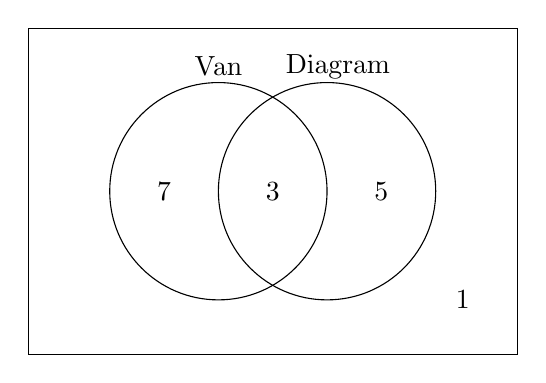
\begin{tikzpicture}[scale=0.69]
	\draw (0,0) rectangle (9,6);
	\draw (3.5,3) circle (2);
	\draw (5.5,3) circle (2);
	
	\node at (3.5,5.3) {Van};
	\node at (5.7,5.3) {Diagram}; 
	
	\node at (2.5,3) {7};
	\node at (4.5,3) {3};
	\node at (6.5,3) {5};
	\node at (8,1) {1};
	\end{tikzpicture}
	\]



% Question 6
\newpage
\question[15] A vendor of a cologne called Sexy Jaguar claims that 20\% of the time `it works' (every time). Suppose you use the cologne 11~times. 
	\begin{enumerate}[(a)]
	\item Find the probability that the cologne works exactly 5 times. 
	\item Find the probability that the cologne works less than 3 times.
	\item Find the probability that the cologne works at most 4 times.
	\item Find the probability that the cologne works at least once. 
	\end{enumerate} \pspace

\sol The cologne either works or not with each use. We assume the cologne works with fixed probability $p= 0.20$. We test the cologne a fixed total of 11~times. We assume each test was independent from the other tests. Then the number of times the cologne works, $X$, is given by the binomial distribution $B(n, p)= B(11, 0.20)$. \pspace

\begin{enumerate}[(a)]
\item 
	\[
	P(X= 5)= 0.0388
	\] \pspace

\item 
	\[
	P(X < 3)= P(X= 0) + P(X= 1) + P(X= 2)= 0.0859 + 0.2362 + 0.2953= 0.6174
	\] \pspace

\item 
	\[
	P(X \leq 4)= P(X < 3) + P(X= 3) + P(X= 4)= 0.6174 + 0.2215 + 0.1107= 0.9496
	\] \pspace

\item 
	\[
	P(X \geq 1)= 1 - P(X= 0)= 1 - 0.0859= 0.9141
	\]
\end{enumerate}



% Question 7
\newpage
\question[15] When you play Monopoly with friends, you only win 40\% of the time. If you lose, you flip the board 90\% of the time in fury. Even if you win, you flip the board in celebration 15\% of the time.
	\begin{enumerate}[(a)]
	\item Find the probability that you flip the board playing Monopoly. 
	\item Find the probability that you do not flip the board playing Monopoly. 
	\item Find the probability that you flip the board or win playing Monopoly. 
	\item Find the probability that if you flipped the board, you had won the game. 
	\end{enumerate} \pspace

\sol 
\begin{enumerate}[(a)]
\item 
	\[
	P(\text{flip})= 0.06 + 0.54= 0.60
	\] \pspace

\item 
	\[
	P(\text{not flip})= 1 - P(\text{flip})= 1 - 0.60= 0.40
	\] \pspace

\item 
	\[
	P(\text{flip or win})= 0.06 + 0.34 + 0.54= 0.94
	\] \pspace

\item 
	\[
	P(\text{won} \;|\; \text{flip})= \dfrac{P(\text{won and flip})}{P(\text{flip})}= \dfrac{0.06}{0.60}= 0.10
	\]
\end{enumerate} \pspace \vfill

		\[
		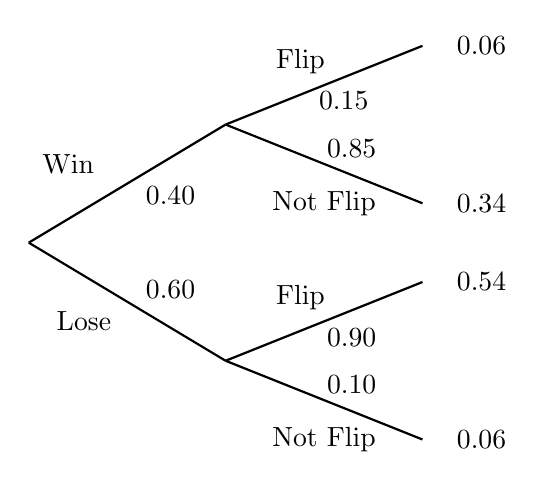
\begin{tikzpicture}[scale= 1.0]
		\def\FirstUpLabel{Win}
		\def\FirstDownLabel{Lose}
		\def\SecondUpLabel{Flip}
		\def\SecondDownLabel{Not Flip}
		\def\Up{$0.40$}
		\def\Down{$0.60$}
		\def\UpUp{$0.15$}
		\def\UpDown{$0.85$}
		\def\DownUp{$0.90$}
		\def\DownDown{$0.10$}
		\def\first{$0.06$}
		\def\second{$0.34$}
		\def\third{$0.54$}
		\def\fourth{$0.06$}
		
		\node at (0.5,1) {\FirstUpLabel};	
		\node at (0.7,-1) {\FirstDownLabel};	
		\node at (1.8,0.6) {\Up};
		\node at (1.8,-0.6) {\Down};
		\draw[thick] (0,0) -- (2.5,1.5);
		\draw[thick] (0,0) -- (2.5,-1.5);
		
		\node at (3.45,2.3) {\SecondUpLabel};
		\node at (3.75,0.5) {\SecondDownLabel};
		\node at (4,1.8) {\UpUp};
		\node at (4.1,1.2) {\UpDown};
		\node at (5.75,2.5) {\first};
		\node at (5.75,0.5) {\second};
		\draw[thick] (2.5,1.5) -- (5,2.5);
		\draw[thick] (2.5,1.5) -- (5,0.5);

		\node at (3.45,-0.7) {\SecondUpLabel};
		\node at (3.75,-2.5) {\SecondDownLabel};
		\node at (4.1,-1.2) {\DownUp};
		\node at (4.1,-1.8) {\DownDown};
		\node at (5.75,-0.5) {\third};	
		\node at (5.75,-2.5) {\fourth};	
		\draw[thick] (2.5,-1.5) -- (5,-0.5);
		\draw[thick] (2.5,-1.5) -- (5,-2.5);
		\end{tikzpicture}
		\]


\end{questions}
\end{document}